  \let\negmedspace\undefined
\let\negthickspace\undefined
\documentclass[journal]{IEEEtran}
\usepackage[a5paper, margin=10mm, onecolumn]{geometry}
\usepackage{lmodern} % Ensure lmodern is loaded for pdflatex
\usepackage{tfrupee} % Include tfrupee package

\setlength{\headheight}{1cm} % Set the height of the header box
\setlength{\headsep}{0mm}     % Set the distance between the header box and the top of the text

\usepackage{gvv-book}
\usepackage{gvv}
\usepackage{cite}
\usepackage{amsmath,amssymb,amsfonts,amsthm}
\usepackage{algorithmic}
\usepackage{graphicx}
\usepackage{textcomp}
\usepackage{xcolor}
\usepackage{txfonts}
\usepackage{listings}
\usepackage{enumitem}
\usepackage{mathtools}
\usepackage{gensymb}
\usepackage{comment}
\usepackage[breaklinks=true]{hyperref}
\usepackage{tkz-euclide} 
\usepackage{listings}                                      
\def\inputGnumericTable{}                                 
\usepackage[latin1]{inputenc}                                
\usepackage{color}                                            
\usepackage{array}                                            
\usepackage{longtable}
\usepackage{multicol}
\usepackage{calc}                                             
\usepackage{multirow}                                         
\usepackage{hhline}                                           
\usepackage{ifthen}                                           
\usepackage{lscape}
\begin{document}

\bibliographystyle{IEEEtran}
\vspace{3cm}

\title{9.3.11}
\author{EE24BTECH11024 - G. Abhimanyu Koushik}
% \maketitle
% \newpage
% \bigskip
{\let\newpage\relax\maketitle}

\renewcommand{\thefigure}{\theenumi}
\renewcommand{\thetable}{\theenumi}
\setlength{\intextsep}{10pt} % Space between text and floats


\numberwithin{equation}{enumi}
\numberwithin{figure}{enumi}
\renewcommand{\thetable}{\theenumi}


\textbf{Question}:\newline
Solve the differential equation $\frac{d^2y}{dx^2} + 1 = 0$ with initial conditions $y\brak{0} = 0$ and $y^{\prime}\brak{0} = 0$
\newline
\textbf{Solution: }
\begin{table}[h!]    
  \centering
  \begin{tabular}[12pt]{ |c| c| c |}
    \hline
    \textbf{Variable} & \textbf{Description} & \textbf{values}\\ 
    \hline
    $\vec{V}$ & Quadratic form of the matrix & $\myvec{1 & 0 \\ 0 & 1} $\\
    \hline
    $\vec{u}$ & Linear coefficient vector & $\myvec{0 \\ 0} $\\
    \hline
    f & constant term & -4 \\ 
    \hline
    $\vec{m}$ & The direction vector of line & $\myvec{1 \\ 0}$\\
    \hline
     $\vec{h}$ & Point on line & \myvec{2 \\ 0} \\
     \hline
\end{tabular}

  \caption{Variables Used}
  \label{tab1.1.2.2}
\end{table}
\newline
Theoritical Solution:\\
Laplace Transform definition\\
\begin{align}
	\mathcal{L}\brak{f\brak{t}} = \int_{0}^{\infty}e^{-st}f\brak{t}dt
\end{align}
Properties of Laplace tranform
\begin{align}
	\mathcal{L}\brak{y^{\prime\prime}} &= s^2\mathcal{L}\brak{y} -sy\brak{0}-y^\prime\brak{0}\\
	\mathcal{L}\brak{1} &= \frac{1}{s}\\
	\mathcal{L}^{-1}\brak{\frac{2}{s^3}} &= x^2u\brak{x}\\
	\mathcal{L}\brak{cf\brak{t}} &= c\mathcal{L}\brak{f\brak{t}}
\end{align}
Applying the properties to the given equation
\begin{align}
	y^{\prime\prime} + 1 &= 0\\
	\mathcal{L}\brak{y^{\prime\prime}} + \mathcal{L}\brak{1} &= 0\\
	s^2\mathcal{L}\brak{y} -sy\brak{0}-y^\prime\brak{0}+\frac{1}{s} &= 0\\
\end{align}
Substituting the initial conditions gives
\begin{align}
	s^3\mathcal{L}\brak{y} + 1 &= 0\\
	\mathcal{L}\brak{y} &= \frac{-1}{s^3}\\
	y &= \mathcal{L}^{-1}\brak{\frac{-1}{s^3}}\\
	y &= \frac{-1}{2}\mathcal{L}^{-1}\brak{\frac{2}{s^3}}\\
	y &= \frac{-1}{2}x^2u\brak{x}
\end{align}
The theoritical solution is 
\begin{align}
	f\brak{x} = \frac{-x^2}{2}u\brak{x}
\end{align}
\newline
Computational Solution:\newline
Consider the given linear differential equation
\begin{align}
	a_{n}y^n + a_{n-1}y^{n-1} + \dots + a_{1}y^\prime + a_{0}y + c = 0
\end{align}
Then
\begin{align}
	y^{\prime}\brak{t} = \lim_{h\to 0}\frac{y\brak{t+h} - y\brak{t}}{h}\\
	y\brak{t+h} = y\brak{t} + hy^{\prime}\brak{t}
\end{align}
Similarly
\begin{align}
	y^{i}\brak{t+h} &= y^{i}\brak{t} + hy^{i+1}\brak{t}\\
	y^{n-1}\brak{t+h} &= y^{n-1}\brak{t} + hy^{n}\brak{t}\\
	y^{n-1}\brak{t+h} &= y^{n-1}\brak{t} + h\brak{-\frac{a_{n-1}}{a_n}y^{n-1}-\frac{a_{n-2}}{a_n}y^{n-2} - \dots -\frac{a_{0}}{a_n}y - \frac{c}{a_n}}
\end{align}
Where i ranges from 0 to $n-1$\\
\begin{align}
	\vec{y}\brak{t+h} = \vec{y}\brak{t} + \myvec{0 & 0 & 0 & 0 & \dots & 0 & 0\\ 0 & 0 & 1 & 0 & \dots & 0 & 0\\0 & 0 & 0 & 1 & \dots & 0 & 0\\\vdots & \vdots & \vdots & \vdots& \ddots & \vdots & \vdots\\
	0 & 0 & 0 & 0 & \dots & 0 & 1\\-\frac{1}{a_n} & -\frac{a_0}{a_n} & -\frac{a_1}{a_n} & -\frac{a_2}{a_n} & \dots & -\frac{a_{n-2}}{a_n} & -\frac{a_{n-1}}{a_n}}\brak{h\vec{y}\brak{t}}\\
	\vec{y}\brak{t+h} = \myvec{1 & 0 & 0 & 0 & \dots & 0 & 0\\ 0 & 1 & h & 0 & \dots & 0 & 0\\0 & 0 & 1 & h & \dots & 0 & 0\\\vdots & \vdots & \vdots & \vdots& \ddots & \vdots & \vdots\\
	0 & 0 & 0 & 0 & \dots & 1 & h\\-\frac{h}{a_n} & -\frac{a_0h}{a_n} & -\frac{a_1h}{a_n} & -\frac{a_2h}{a_n} & \dots & -\frac{a_{n-2}h}{a_n} & 1-\frac{a_{n-1}h}{a_n}}\brak{\vec{y}\brak{t}}
\end{align}
Discretizing the steps gives us
\begin{align}
	\vec{y}_{k+1} = \myvec{1 & 0 & 0 & 0 & \dots & 0 & 0\\ 0 & 1 & h & 0 & \dots & 0 & 0\\0 & 0 & 1 & h & \dots & 0 & 0\\\vdots & \vdots & \vdots & \vdots& \ddots & \vdots & \vdots\\
	0 & 0 & 0 & 0 & \dots & 1 & h\\-\frac{h}{a_n} & -\frac{a_0h}{a_n} & -\frac{a_1h}{a_n} & -\frac{a_2h}{a_n} & \dots & -\frac{a_{n-2}h}{a_n} & 1-\frac{a_{n-1}h}{a_n}}\brak{\vec{y}_{k}}
\end{align}
where $k$ ranges from 0 to number of data points with $y^{i}_0$ being the given initial condition and vector $\vec{y}_0 = \myvec{c\\y\brak{0}\\y^\prime\brak{0}\\\vdots\\y^{n-1}\brak{0}}$\\
For the given question\\
\begin{align}
	\vec{y}_{k+1} = \myvec{1 & 0 & 0\\ 0 & 1 & h\\ -h & 0 & 1}\vec{y}_k
\end{align}
Record the $y_k$ for 
\begin{align}
x_k =lowerbound+kh
\end{align}
and then plot the graph. The result will be as given below.
\begin{figure}[h!]
   \centering
   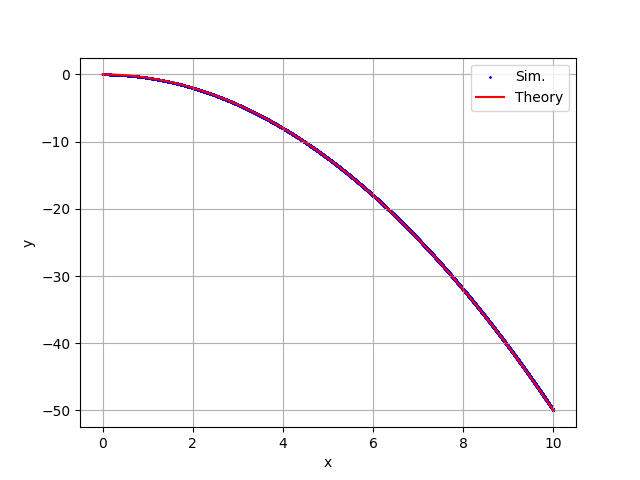
\includegraphics[width=\columnwidth]{figs/fig.png}
   \caption{Comparison between the Theoritical solution and Computational solution}
   \label{stemplot}
\end{figure}
\end{document}  
